Zusammen mit der für den jeweiligen Einsatzzweck benötigten Peripherie bilden sowohl ein Arduino Nano als auch ein CAN-Bus Modul den Grundstein für die zur Steuerung des Bootes benötigte Elektronik.\\

\begin{minipage}{7cm}
    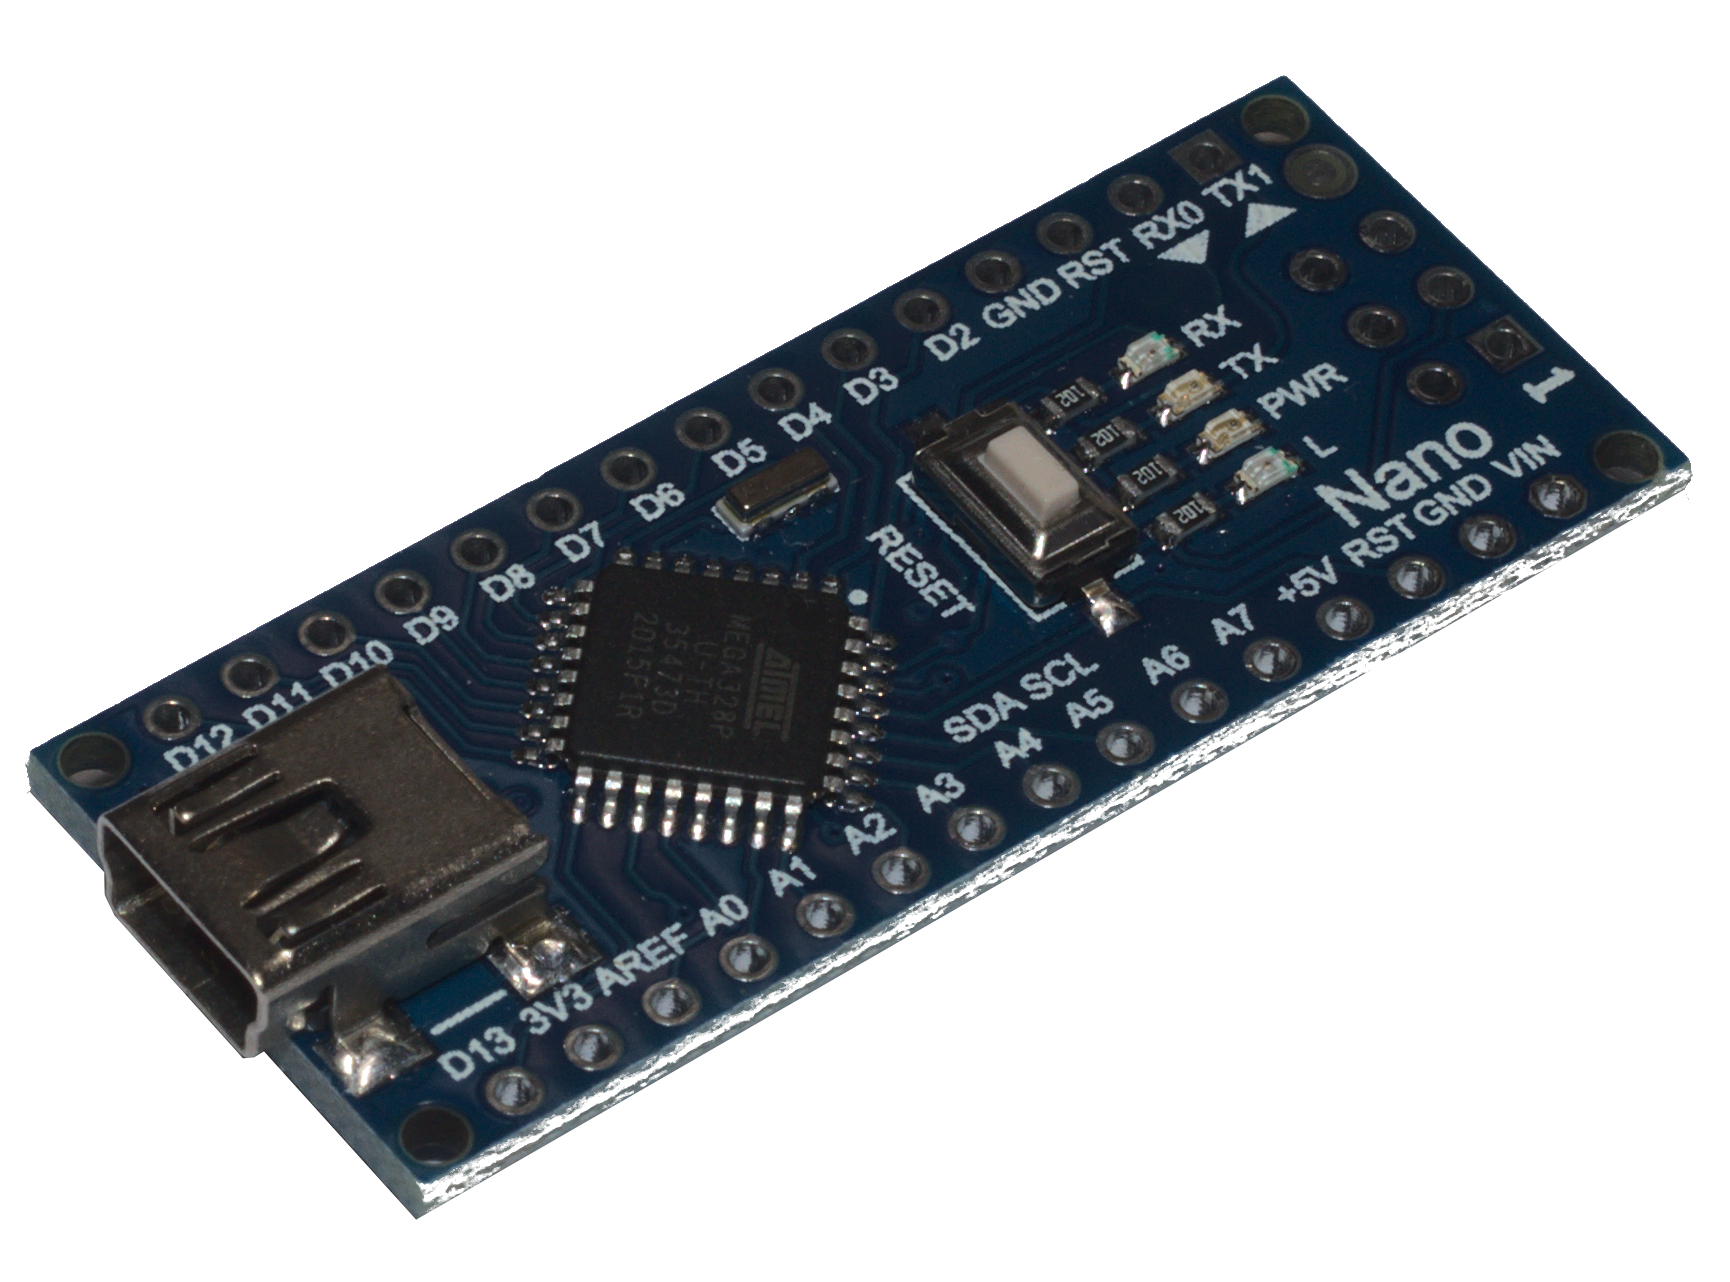
\includegraphics[width=\textwidth]{Fotos/Arduino_Nano.png}
    \captionof{figure}{Arduino Nano}
\end{minipage}
\begin{minipage}{7cm}
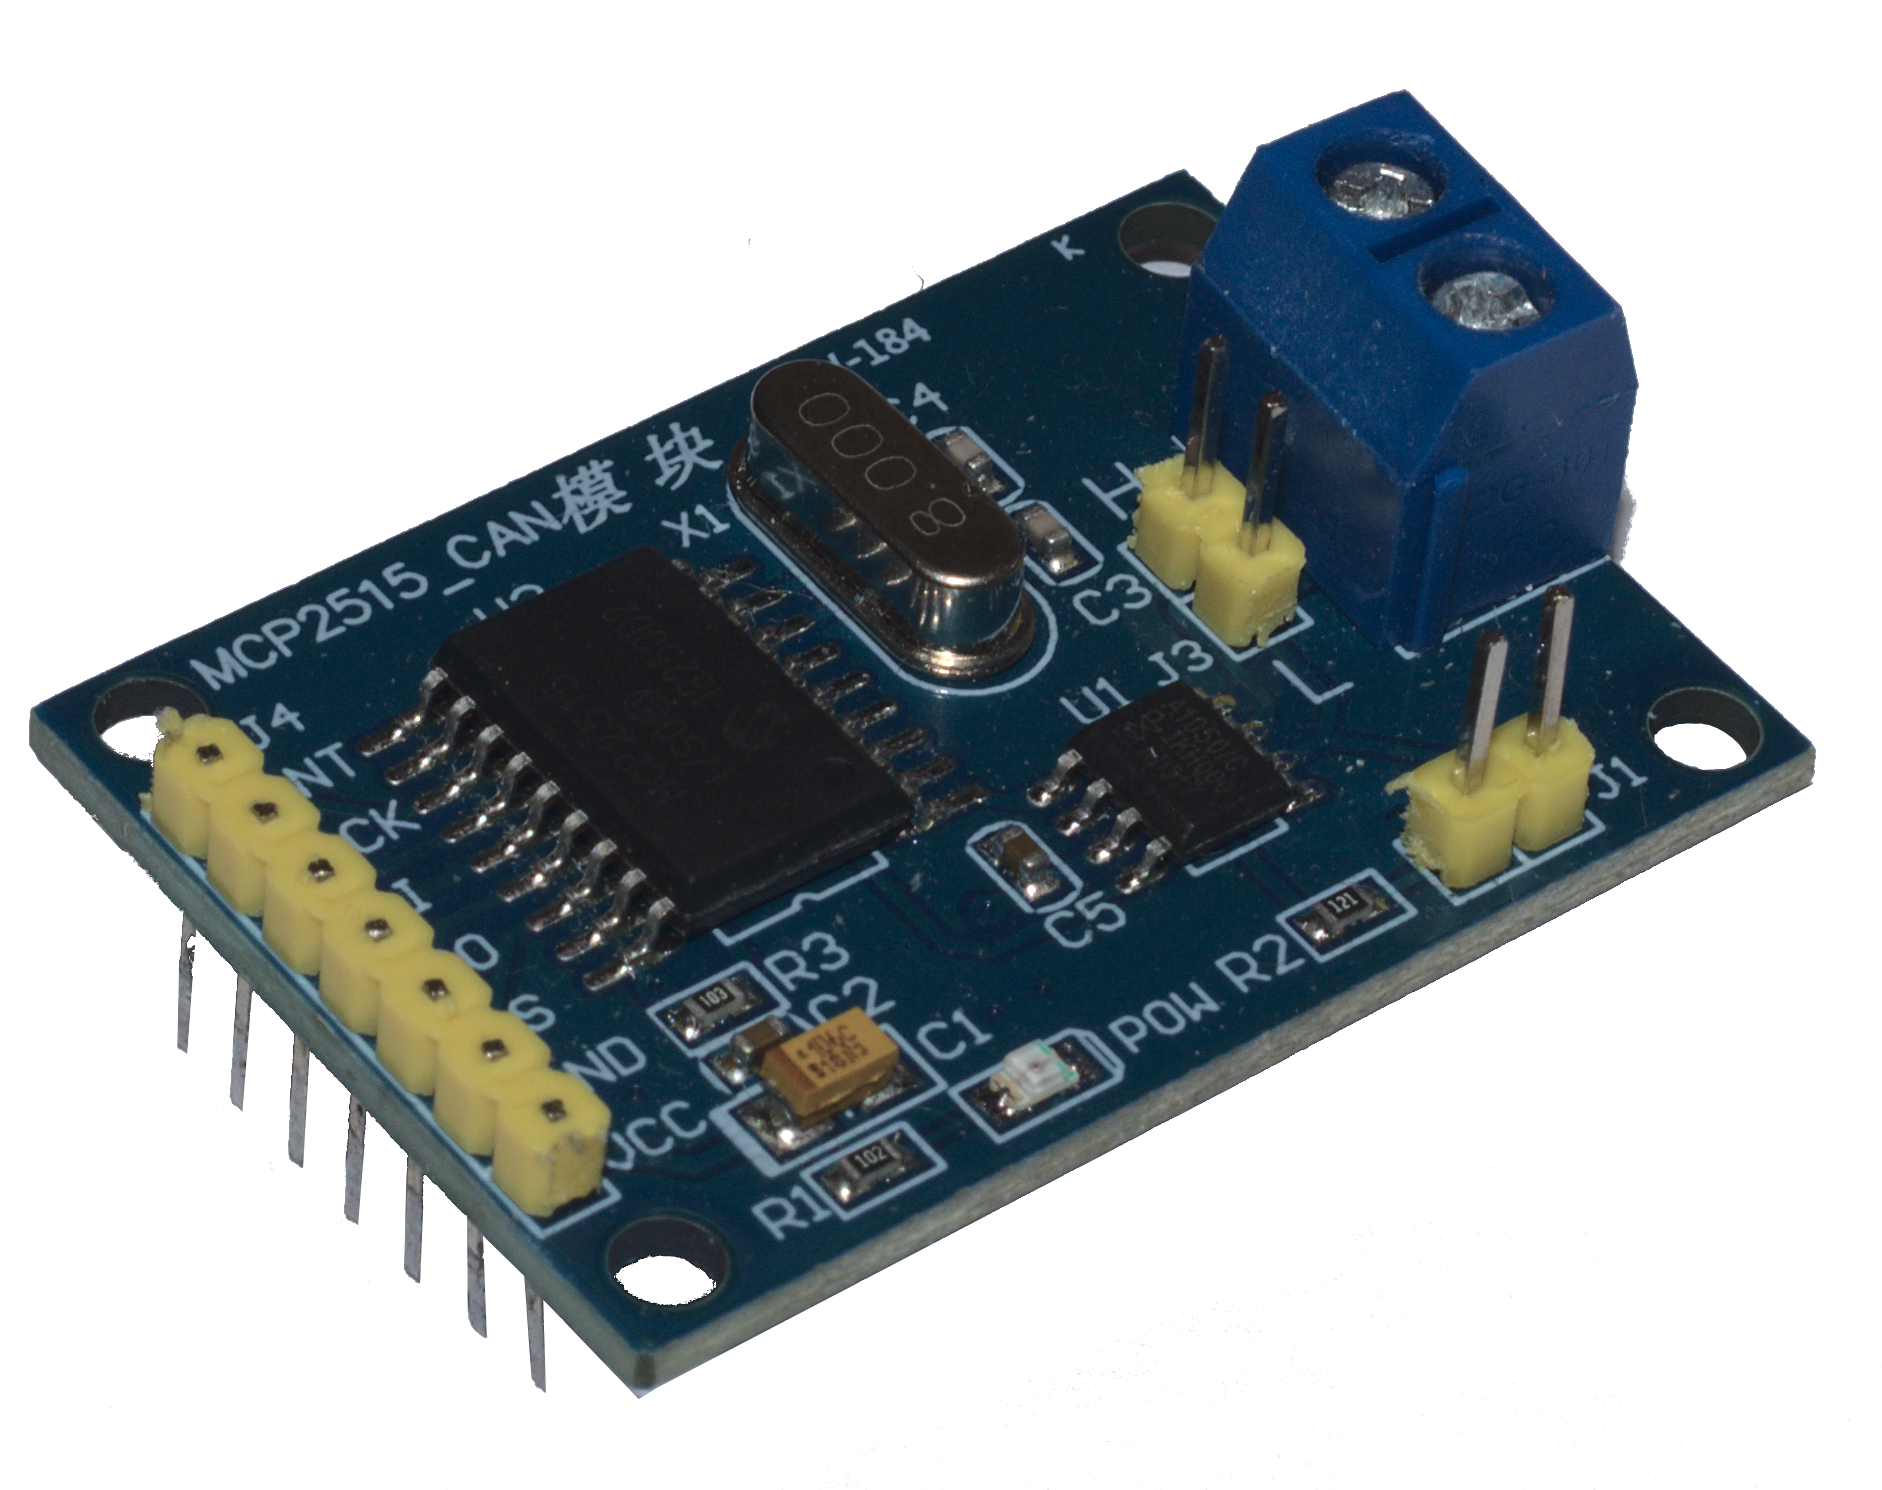
\includegraphics[width=\textwidth]{Fotos/CAN_BUS_Shield.png}
\captionof{figure}{CAN-Bus Modul}
\end{minipage}
\section{Übertragungsmedium CAN-Bus}
\subsection{Gründe für die Verwendung}
Um eine zuverlässige Übertragung der Regelparameter für unsere Motoren sowie Servos garantieren zu können, wurde für deren Übertragung ein aus der Automobilbranche bekanntes Übertragungsmedium verwendet, der CAN-Bus. 
Neben seiner Robustheit trotz relativ hoher Übertragungsgeschwindigkeit, war es vorallem sein dezentraler Aufbau, der ihn für unseren Anwendungszweck optimal gemacht hat.

\newpage

\subsection{Verwendete Adressen}
\begin{table}[h]
    \begin{tabular}{|l|l|l|l|}
        \hline
    Name                              & CAN-ID & Info         & Länge \\\hline
    CONTROL\_MOTORS\_SERVOS  & 0xC0   & Gas-\& Lenkerstellung & 3     \\
    INFOS\_LOWER\_CONTROLLER & 0xC1   & Telemetriedaten Motor unten  & 6     \\
    INFOS\_BACK\_CONTROLLER  & 0xC3   & Telemetriedaten Motor hinten & 6     \\
    BATTERY\_TEMPS           & 0xE0   & Akku-Temperaturen            & 8    \\\hline
    \end{tabular}
    \caption{Verwendete CAN-Bus Adressen}
\end{table}
